
% This LaTeX was auto-generated from MATLAB code.
% To make changes, update the MATLAB code and republish this document.

\documentclass{article}
\usepackage{graphicx}
\usepackage{color}

\sloppy
\definecolor{lightgray}{gray}{0.5}
\setlength{\parindent}{0pt}

\begin{document}

    
    \begin{verbatim}
data=Euler(0,1,0,0.1);
plot(data(:,1),data(:,2))
hold on
data=RK4(0,1,0,0.1)
plot(data(:,1),data(:,2))
plot(linspace(0,1),y(linspace(0,1)))
%Adds labels and saves the image
legend({'Euler Method','Runge-Kutta Method','y(x)'},'location',...
    'northeast')
xlabel('x')
ylabel('y')
print('Image_1_1','-depsc')

function data = Euler(x_0,x_n,y_0,h)
%Creates a table to be filled
    data=zeros(ceil((x_n-x_0)/h)+1,5);
    data(1,:)=[x_0,y_0,y(x_0),y_0-y(x_0),0];
    counter=2;
%Iterates through the rows filling them
    while counter<=ceil((x_n-x_0)/h)+1
        data(counter,:)=[(counter-1)*h+x_0,...
            data(counter-1,2)+h*f((counter-2)*h+x_0,data(counter-1,2)),...
            y((counter-1)*h+x_0),...
            data(counter-1,2)+h*f((counter-2)*h+x_0,data(counter-1,2))-...
            y((counter-1)*h+x_0),...
            (data(counter-1,2)+h*f((counter-2)*h+x_0,data(counter-1,2))-...
            y((counter-1)*h+x_0))/data(counter-1,4)];
        counter=counter+1;
    end
end

function data = RK4(x_0,x_n,y_0,h)
%Follows a similar idea to the Euler function
    data=zeros(ceil((x_n-x_0)/h)+1,5);
    data(1,:)=[x_0,y_0,y(x_0),y_0-y(x_0),0];
    counter=2;
    while counter<=ceil((x_n-x_0)/h)+1
        k1=h*f((counter-2)*h+x_0,data(counter-1,2));
        k2=h*f((counter-2+1/2)*h+x_0,data(counter-1,2)+1/2*k1);
        k3=h*f((counter-2+1/2)*h+x_0,data(counter-1,2)+1/2*k2);
        k4=h*f((counter-2+1)*h+x_0,data(counter-1,2)+k3);
        data(counter,:)=[(counter-1)*h+x_0,...
            data(counter-1,2)+1/6*(k1+2*k2+2*k3+k4),...
            y((counter-1)*h+x_0),...
            data(counter-1,2)+1/6*(k1+2*k2+2*k3+k4)-y((counter-1)*h+x_0),...
            (data(counter-1,2)+1/6*(k1+2*k2+2*k3+k4)-y((counter-1)*h+x_0))/...
            data(counter-1,4)];
        counter=counter+1;
    end
end

%These two functions were created to stop repeatedly defining them in the
%above
function z = f(x,y)
    z = -4*y+4*exp(-2*x);
end

function z = y(x)
    z= -2*exp(-4*x)+2*exp(-2*x);
end
\end{verbatim}

        \color{lightgray} \begin{verbatim}
data =

            0            0            0            0            0
          0.1      0.29671      0.29682  -0.00011492         -Inf
          0.2      0.44183      0.44198  -0.00014739       1.2826
          0.3      0.49509      0.49523   -0.0001405      0.95326
          0.4      0.49475      0.49486  -0.00011766      0.83745
          0.5        0.465      0.46509   -9.095e-05      0.77297
          0.6      0.42089      0.42095  -6.6062e-05      0.72636
          0.7      0.37153      0.37157  -4.5243e-05      0.68486
          0.8      0.32224      0.32227   -2.896e-05       0.6401
          0.9      0.27593      0.27595  -1.6849e-05      0.58181
            1      0.23403      0.23404  -8.2276e-06      0.48831

\end{verbatim} \color{black}
    
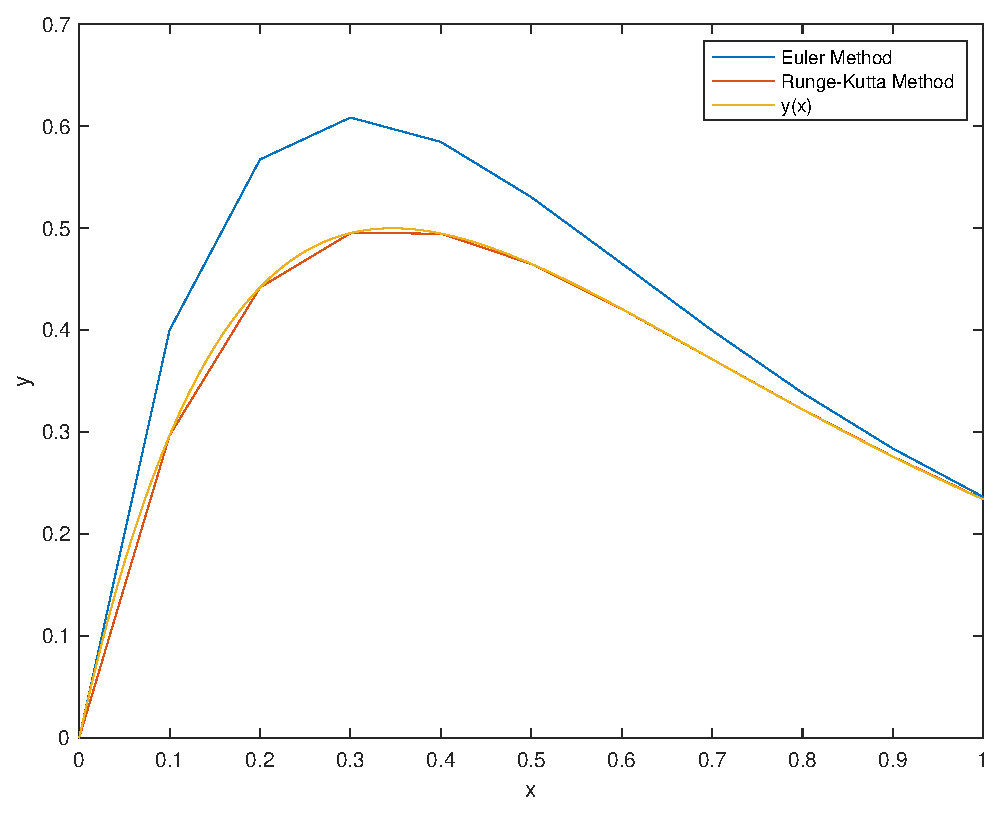
\includegraphics [width=4in]{RevampQuestion_1_2_01.eps}



\end{document}
    
